\section{Experiments}

This section contains the key takeaways of seven experiments about timing attacks. The first performed by Kocher, and the other six by Brumley and Boneh.

Together with this report, we made available some source code files that allow to simulate the timing attacks discussed so far. We summarize the implementation at the end of this section.

\subsection{Kocher's experiment}

In his article, Kocher described an experiment in which he performed several attacks against modular exponentiation that precomputed two exponent bits per iteration. There are two key points that we can grasp from his experiment.

First of all, that timing attacks are computationally quite easy to perform, and thus practical. This because the attacker only needs to evaluate four times the number of operations done by the victim (without counting incorrect guesses).

Second, that the theoretical probability of a correct guess (described in \Cref{subsub:guess}) is significantly close to the empirical one computed in the experiment. Specifically, with an expected probability of $\sim 0.84$, among 2450 trials, $~88.5\%$ of them were correct guesses, using a sample size $s = 250$ for each trial.

\subsection{Brumley and Boneh's experiments}

Brumley and Boneh carried out six experiments:

\begin{enumerate}

  \item First, they provided a formula to approximate how many decryption operations are needed to recover an RSA factor, given a neighborhood size $n$ and a sample size $s$.
During an attack, for every bit of $q$, they measured the decryption time for a neighborhood of values $g, g + 1, \dots, g + (n - 1)$. In addition, for each value $g + i$ in a neighborhood, they performed $s$ decryption operations and took the average among decryption times. Thus the formula that estimates the number of decryptions required is the following: $$ 2ns \cdot log_2 \left( N/4 \right), $$
where $N$ is the public RSA modulus.

  \item Second, they tried to recover three distinct keys, showing a correlation between keys and the zero-one gap created by the differences $|T_g - T'_g|$ when a bit of $q$ is 0 or 1. As we already mentioned in \Cref{subsec:openssl}, the larger the gap, the greater the chance that $q$ is $0$. Another fact that was pointed out, was that the zero-one gap can be expanded by increasing the neighborhood size, reducing the chance of error, especially when bits hard to guess are encountered.

  \item Third, they concluded that users of binary crypto libraries should be aware of the compile-time options, and exact execution environment to understand the risk of their timing attack. This because slight changes to them, in combinations of system and compilation settings, can lead to huge changes in zero-one gap estimations.

  \item Fourth, they implemented a minor patch for OpenSSL that was accepted for future incorporation. Their goal was to increase the evidence in suggesting that developers should be careful in relying on timing attack tests. Despite their patch decreases the zero-one gap, others may lead to an increase in it.

  \item Fifth, they showed that local network timing attacks are practical. They also provided an upper bound of approximately $1$ms for the zero-one gap to judge a network vulnerable.

  \item Sixth, they highlighted the difficulty in estimating the minimum number of decryption operations that a successful attack would require. They performed two attacks against two networks that were equal for the majority of the involved parameters except they were distinct in the number of network switches. Surprisingly, the network with less switches (only one switch) brought to an average zero-one gap smaller than the average zero-one gap encountered in the other network. Nevertheless, an important aspect of this experiment is that the attacks worked even in a large network.

\end{enumerate}


\subsection{Timing attack simulations}

This report comes along with some source code files written in Python programming language that aim to ease timing attack simulations.
There are four main files:
\begin{itemize}
  \item kocher\_main.py;
  \item TimingAttackModule.py\footnote{Professor Michele Boreale provided it.};
  \item brumley\_and\_boneh\_main.py;
  \item utilities.py.
\end{itemize}

Kocher's timing attack can be simulated with kocher\_main.py that simply follows all the steps described in \Cref{alg:two} relying on TimingAttackModule.py to emulate the behaviour of an RSA based device that uses $\modexp$ in its plain form.

The attack designed by Brumley and Boneh can be performed using brumley\_and\_boneh.py. This file implements two classes, Device and Attacker.
The class Device emulates an RSA based device that behaves like it is making use of all the $\modexp$ enhancements described in \Cref{sec:technical}, namely Chinese Remainder, Sliding Windows, Montgomery multiplication, and Karatsuba's algorithm.
An instance of the class Device can differ from another by:

\begin{itemize}
  \item number of bits of the public modulus;
  \item initial seed of the underneath Random Number Generator;
  \item presence or absence of the blinding technique.
\end{itemize}

In addition, the actions allowed by an instance of the class Device are the following:

\begin{itemize}
  \item to retrieve the public Montgomery coefficient;
  \item to retrieve the public modulus;
  \item to run a decryption, given any ciphertext.
\end{itemize}

An attacker can be initialized with the class Attacker that requires an instance of the class Device, as well as other three pieces of information:

\begin{itemize}
  \item the number of bits per modulus factor (assumed equal for both factors);
  \item the public modulus;
  \item the public Montgomery coefficient.
\end{itemize}

Once an attacker is defined, he can guess the target exponent providing a floating point threshold. This threshold is required by the attack described in \Cref{alg:three} for the time variations in order to distinguish different bits of the minimum modulus factor. Moreover, he can also draw a graph representing time variations in function of the guessed bitsof the exponent. This helps to visually recognize a suitable threshold for the attack.

An example of a simulation of Brumley and Boneh's timing attack is the following:
\begin{lstlisting}{backgroundcolor}[language=Python]
    device = Device(num_bits=64, seed=42, blinding=False)
    attacker = Attacker(device)
    g = attacker.guess()
    attacker.plot_last_guess()
\end{lstlisting}

\begin{figure}[h]
  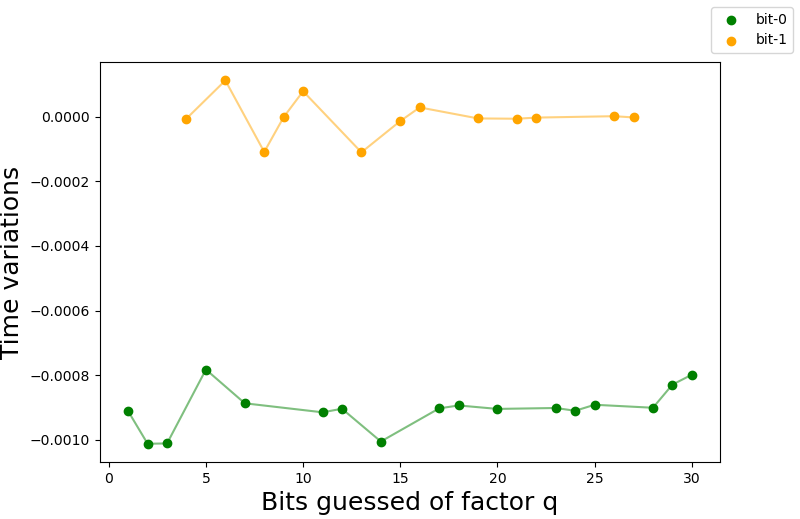
\includegraphics[width=0.65\textwidth]{figures/brumley_and_boneh_output_example}
\end{figure}

During a guess, the attacker queries several times the given device logging elapsed times to perform the attack. But how does the given device simulate the times required by a decryption in an OpenSSL server?
Using the same notation as in \Cref{alg:three}, let $u$ be an integer such that $u =: g \cdot R^{-1} \bmod n$. Now, when the attacker performs a decryption providing $u$ to the device, the latter behaves as follows:
\begin{enumerate}
  \item converts the input $u$ in its Montgomery form (yielding $g$);
  \item initializes elapsed times $t_q := 0$, and $t_p := 0$;
  \item checks if $g < q$, and if true:
    \begin{itemize}
      \item $t_q = t_q + 1000$ (many Montgomery reductions);
      \item $t_q = t_q + 100$ (normal multiplication routine);
    \end{itemize}
  \item[] otherwise ($g \ge self.q$):
    \begin{itemize}
      \item $t_q = t_q + 10$ (few Montgomery reductions);
      \item $t_q = t_q + 10$ (Karatsuba multiplication routine);
    \end{itemize}
  \item repeats step 3. with $p$ (updating $t_p$);
  \item makes the system do nothing for $\frac{\mathcal{N}(t_q + t_p,\ 5)}{1e6}$ seconds.
\end{enumerate}

Magic numbers in step 3. are made up aiming only to follow a consistency in elapsed times.

Another example, that differs from the previous one only by the presence of the blinding technique is the following:

\begin{lstlisting}{backgroundcolor}[language=Python]
    device = Device(num_bits=64, seed=42, blinding=$\textbf{True}$)
    attacker = Attacker(device)
    g = attacker.guess()
    attacker.plot_last_guess()
\end{lstlisting}

\begin{figure}[h]
  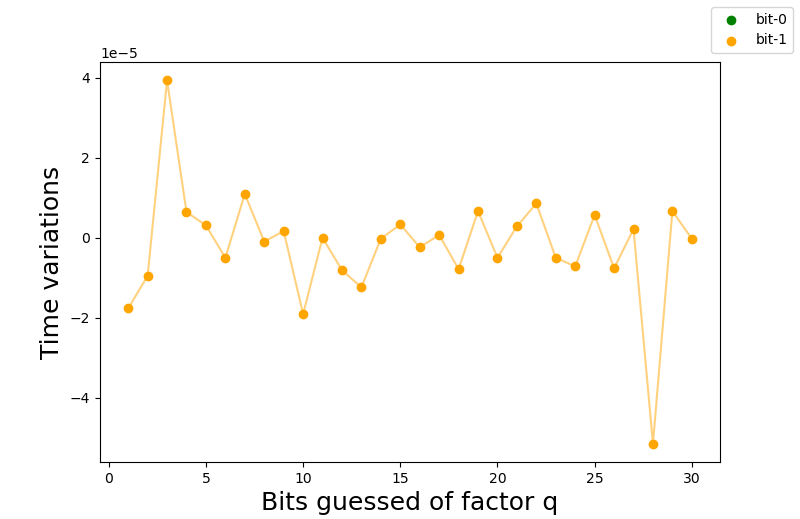
\includegraphics[width=0.65\textwidth]{figures/brumley_and_boneh_output_example_with_blinding}
\end{figure}

Most of the used routines are stored in utilities.py source file. The main functions are dependent on each other, and allow generating RSA factors, generate random prime numbers in a given range, and perform a Miller-Rabin test\cite{bib:boreale}.

%----------------------------------------------------------------------------------------

